\begin{frame}{Margit Sandemo, 1924--2018}
    \note{\tiny{
    Introducing the mastermind behind the book series: \emph{Margit Sandemo}.
    She brought to life the captivating tale of the cursed family we delve into today.
 \begin{itemize}
\item Born in 1924 and living until 2018, Margit's life was deeply intertwined with our ÍSKISUR project.
\item With a literary heritage, including a poet for a father, she added her own remarkable chapters to the family legacy.
\item She started her writing journey at 40, proving it's never too late to follow your dreams.
\item Since the 1980s, her books were favorites in the Nordics, showcasing her storytelling talent.
\item Her major works include: \emph{The Legend of the Ice People}, our key focus. \emph{The Warlock} — exploring a lineage of witches. \emph{The Legend of the Realm of Light} — a sequel to the Ice People's tales.
\item Margit had a knack for blending history with fiction, transporting readers to rich and vivid worlds.
\item Her stories not only entertained but also spotlighted the wonders of Iceland to a global audience by weaving into her tales that Lucifer found a home in Dimmuborgir.
\item Her dedication to the Ice People for two decades speaks volumes about her passion and creativity.
\end{itemize}

}}

    \begin{columns}[T]
        \begin{column}{0.6\textwidth}
            \begin{itemize}
                \item Norwegian-Swedish author
                \item Father was a Norwegian poet, Anders Underdal
                \item Claimed lineage to Nobel Prize-winning author Bjørnstjerne Bjørnson
                \item First published at forty years old
                \item Best-selling author in the Nordic countries since the 1980s
            \end{itemize}
            \vfill
            \begin{scriptsize}
                \begin{table}
                    \begin{tabular}{rcc}
                        \textbf{Notable Book Series}     & \textbf{Years} & $n$ \\ \midrule
                        The Legend of the Ice People     & 1982--89       & 47  \\
                        The Warlock                      & 1991--94       & 15  \\
                        The Legend of the Realm of Light & 1995--99       & 12
                    \end{tabular}
                \end{table}
            \end{scriptsize}
        \end{column}
        \begin{column}{0.4\textwidth}
            \centering
            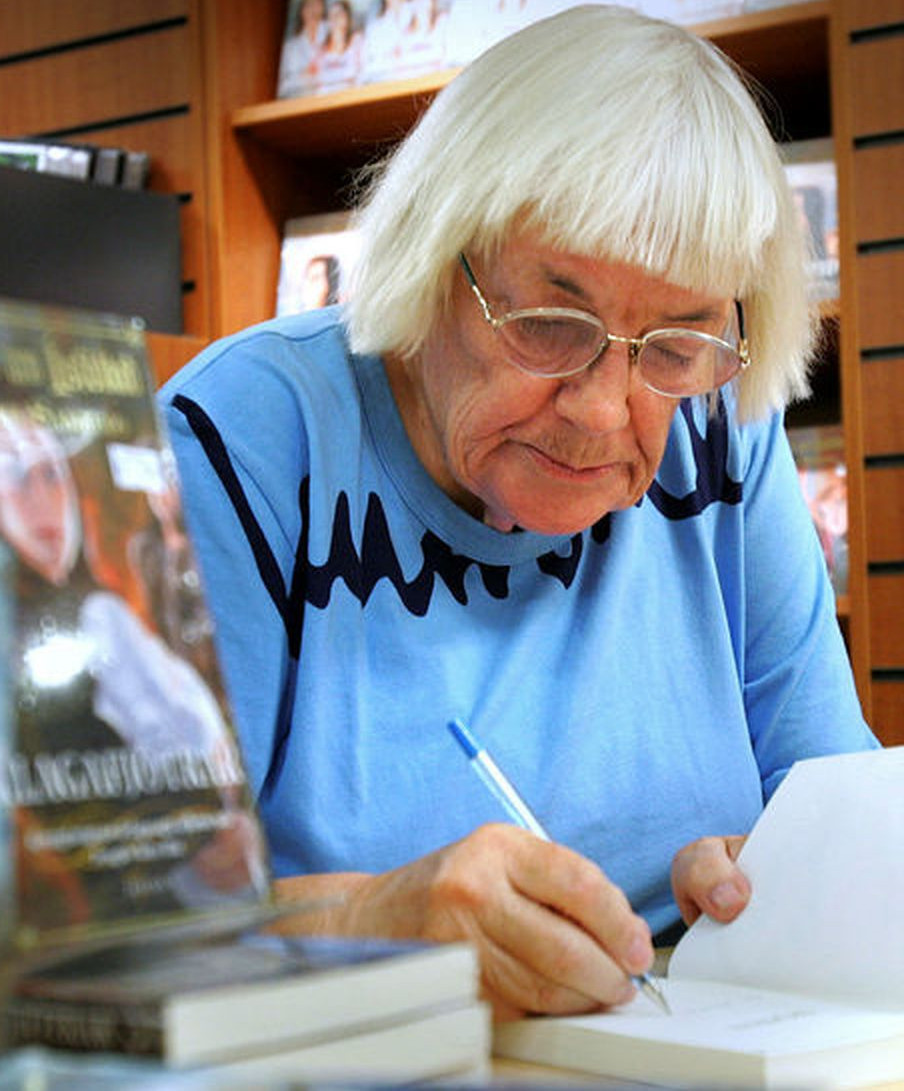
\includegraphics[width=\textwidth]{../rek-data-beers/figures/margit_sandemo}
            \begin{tiny}
                mbl.is/Þorvaldur Örn Kristmundsson
            \end{tiny}

            \vfill
            Margit signing \emph{Álagafjötrar} in Eymundsson, 2007
        \end{column}
    \end{columns}
\end{frame}

\begin{frame}{Publications}

    \note{\scriptsize
    The scatter plot tracks Margit's book publications in Iceland through \emph{Prenthúsið} over a busy 8 years.

    Key insights:
    \begin{itemize}
        \item Margit's output was impressive: 47 books in 8 years, which means a new book every 8-9 weeks, typically released on Tuesdays.
        \item She often stuck to a 14-chapter structure for most books.
        \item As the series progressed, the books got shorter, perhaps hinting at her comments about the narrative challenge in her epilogue,
        \emph{Is There Anybody Out There?}.
        \item Ingibjörg Jónsdóttir began translating the series in 1982, covering the first 33 books. Sadly, she passed away in 1986.
        Ingibjörg Briem then translated the remaining 14.
    \end{itemize}
}
    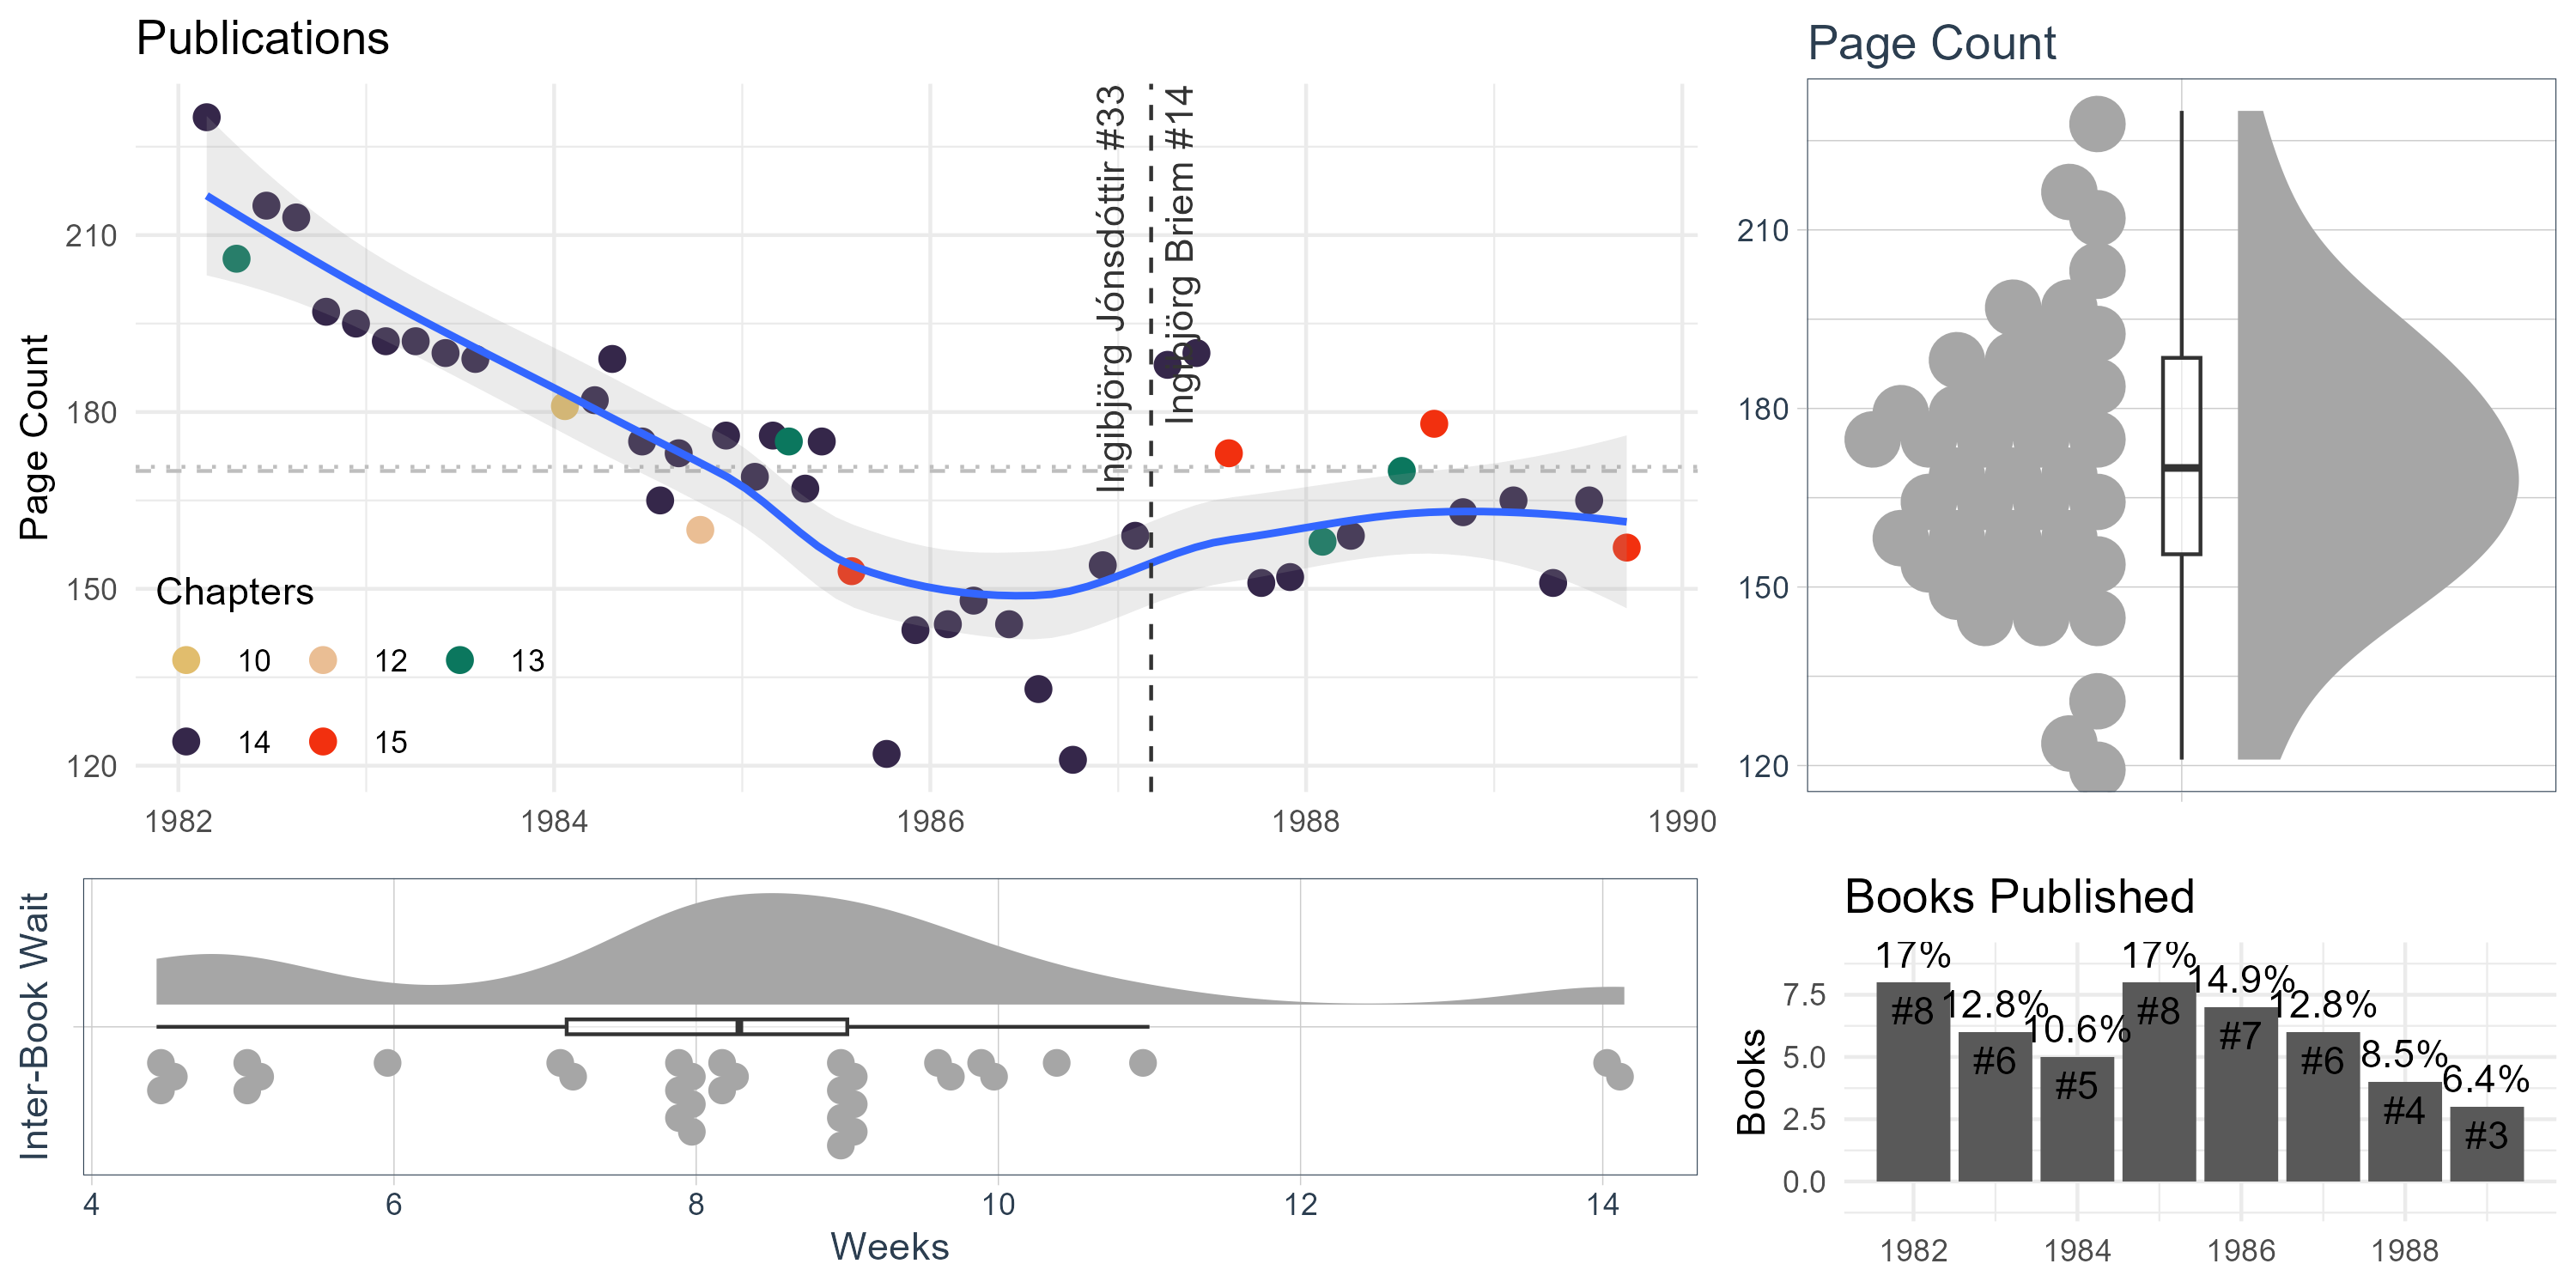
\includegraphics[width=\textwidth]{../rek-data-beers/R/figures/margit_count}
    \vspace{-24pt}
    \begin{itemize}
        \item 47 books, 652 chapters, 8,023 pages, 8 years
        \item Average book length: 170 pages (avg. 13.9 chapters)
        \item Released 1 book every 2 months (avg. 57.9 days), usually on Tue.
    \end{itemize}
\end{frame}
